% Created 2016-04-14 Thu 14:42
\documentclass[10pt,t,a4paper]{beamer}
\usepackage[utf8]{inputenc}
\usepackage[T1]{fontenc}
\usepackage{fixltx2e}
\usepackage{graphicx}
\usepackage{grffile}
\usepackage{longtable}
\usepackage{wrapfig}
\usepackage{rotating}
\usepackage[normalem]{ulem}
\usepackage{amsmath}
\usepackage{textcomp}
\usepackage{amssymb}
\usepackage{capt-of}
\usepackage{hyperref}
\usetheme{BTH_msv}
\author{Mikael Svahnberg\thanks{Mikael.Svahnberg@bth.se}}
\date{2016-04-06}
\title{Design Patterns}
\subtitle{\texttt{PA14[13]5}}
\hypersetup{
 pdfauthor={Mikael Svahnberg},
 pdftitle={Design Patterns},
 pdfkeywords={},
 pdfsubject={},
 pdfcreator={Emacs 25.1.50.1 (Org mode 8.3.4)}, 
 pdflang={English}}
\begin{document}

\maketitle

\section{Upload GoF}
\label{sec:orgheadline19}
\begin{frame}[label={sec:orgheadline1}]{Gang of Four Design Patterns and Architecture Patterns}
\begin{itemize}
\item Architecture
\begin{itemize}
\item Layered
\item MVC
\end{itemize}
\item Design Patterns
\begin{itemize}
\item Observer
\item Singleton
\item Strategy
\item State
\item Abstract Factory
\end{itemize}
\end{itemize}
\end{frame}
\begin{frame}[label={sec:orgheadline2}]{Layered}
\begin{itemize}
\item Problem: \emph{You have groups of subtasks that depend on other subtasks at different levels of abstractions}
\item Solution: \emph{Put the subtasks into \alert{layers}, each representing a specific level of abstraction}
\begin{itemize}
\item Minimise connections between layers (low coupling)
\item Assign a clear responsibility to each layer (high cohesion)
\end{itemize}
\item Examples: Thee Tier Architecture, Windows 2000 Architecture
\end{itemize}
\end{frame}
\begin{frame}[label={sec:orgheadline3}]{Example: Thee Tier Architecture}
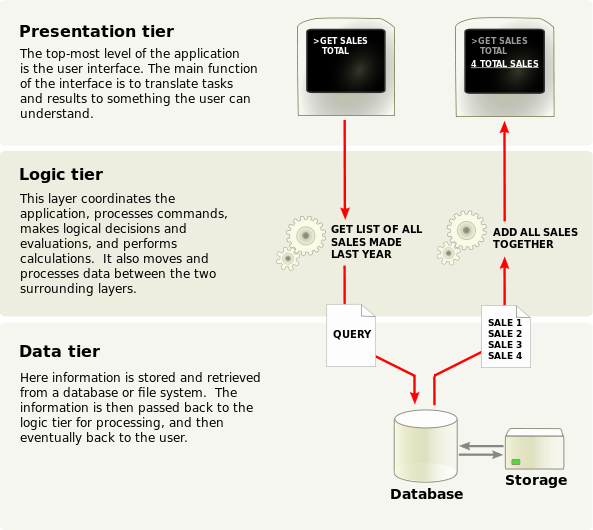
\includegraphics[height=6cm]{./IThreeTierArchitecture.png}
\end{frame}
\begin{frame}[label={sec:orgheadline4}]{Example: Windows 2000 Architecture}
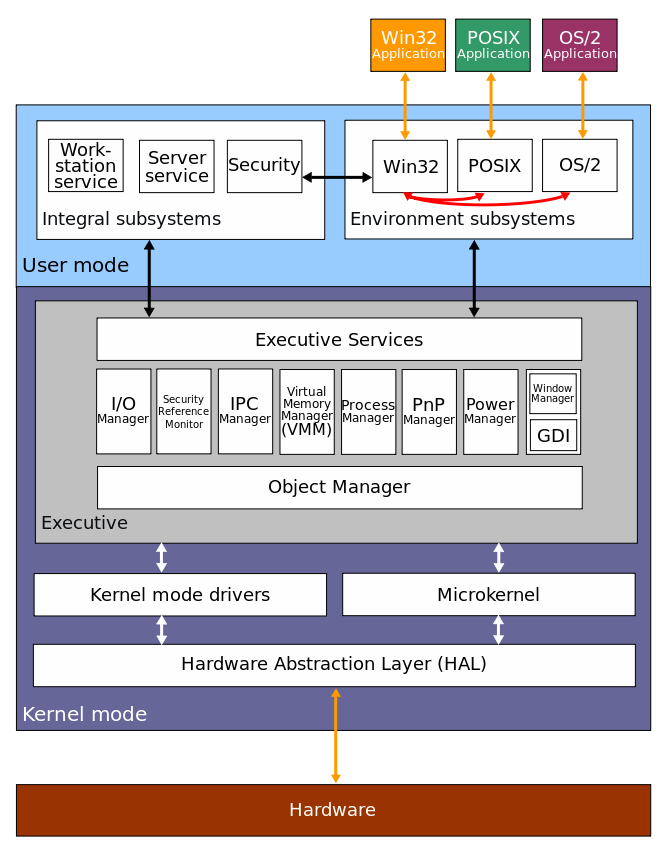
\includegraphics[height=6cm]{./IWindows_2000_architecture.png}
\end{frame}
\begin{frame}[label={sec:orgheadline5}]{Model View Controller: MVC}
\begin{itemize}
\item Problem: \emph{You have an interactive application. How should you divide responsibilities for \alert{presenting}, \alert{managing}, and \alert{storing} data?}
\item Solution: \emph{Divide your system into three parts:}
\begin{itemize}
\item \alert{Model}: Maintain persistency and consistency of the data
\item \alert{View}: Presentation of the data (may be more than one view)
\item \alert{Controller}: Handle user input and manage business rules
\end{itemize}
\item Example: Thee Tier Architecture
\end{itemize}
\end{frame}
\begin{frame}[label={sec:orgheadline6}]{Example: Thee Tier Architecture}
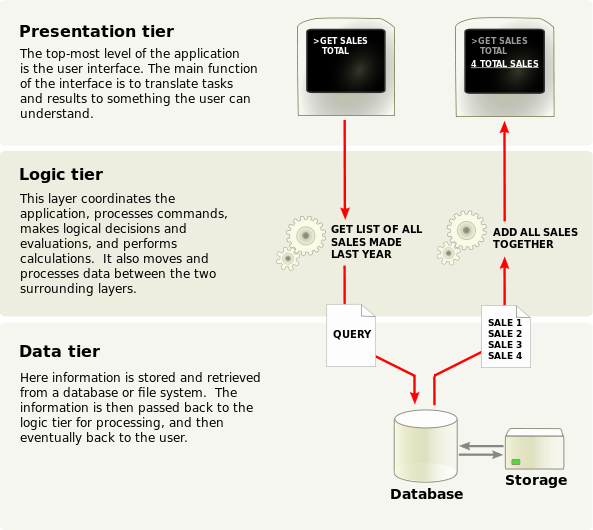
\includegraphics[height=6cm]{./IThreeTierArchitecture.png}
\end{frame}
\begin{frame}[label={sec:orgheadline7}]{Observer}
\begin{itemize}
\item Problem: \emph{How should one object (A) keep track of the state of another object (B)?}
\item Solution: \emph{Give B a pointer to A and ask it to notify when there are changes.}
\item Illustration:
\end{itemize}
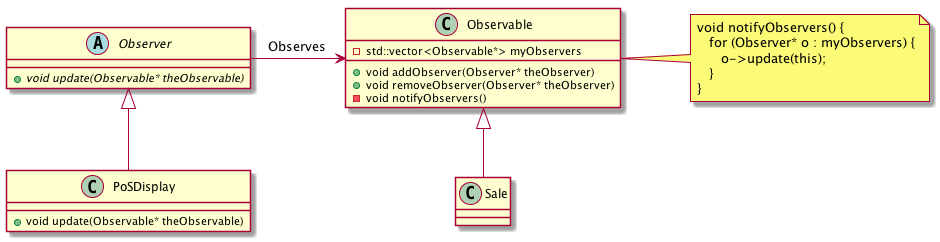
\includegraphics[width=.9\linewidth]{FObserver.png}
\end{frame}
\begin{frame}[label={sec:orgheadline8}]{Java Problem 1: Multiple Inheritance}
\begin{itemize}
\item Problem:  What if you are already extending something? Multiple inheritance is not possible in Java.
\item Solution:
\begin{itemize}
\item re-implement all methods of Observable :-(
\end{itemize}
\end{itemize}
\end{frame}
\begin{frame}[label={sec:orgheadline9}]{Java Problem 2: Observe multiple observables}
\begin{itemize}
\item Problem: What if you want to observe many things
\item Solution:
\begin{itemize}
\item One giant switch/case statement
\item Inner Classes
\item Anonymous Inner Classes
\item Lambda function
\end{itemize}
\end{itemize}
\end{frame}
\begin{frame}[fragile,shrink=15,label={sec:orgheadline10}]{Java Problem 2, Alternative 1}
 \begin{verbatim}
// Alternative 1: Inner Classes
// ---

class DictionaryView {
    public MyFancyView(DictionaryObservable theDictObs, BannerAdObservable theAdObs) {
	theDictObs.addObserver(new DictObserver());
	theAdsObs.addObserver(new AdObserver());
    }

    private class DictObserver implements DictionaryObserver {
       public void update(DictionaryObservable dict) {
	// Logic for updates on Dictionary in update method
       }
    }

    private class AdObserver implements BannerAdObserver {
       public void update(BannerAdObservable banner) {
	// Logic for updates on Banner Ads in update method
       }
    }
}
\end{verbatim}
\end{frame}
\begin{frame}[fragile,shrink=20,label={sec:orgheadline11}]{Java Problem 2, Alternative 2}
 \begin{verbatim}
// Alternative 2: Anonymous Inner Classes
// ---

class DictionaryView {
    public MyFancyView(DictionaryObservable theDictObs, BannerAdObservable theAdObs) {
	theDictObs.addObserver(new DictionaryObserver() {
	  @override
	  public update(DictionaryObservable dict) {
	    // Logic for updates on Dictionary in update method
	  }
	});
	theAdsObs.addObserver(new AdObserver()); // Modify this in the same way
    }
}
\end{verbatim}
\end{frame}
\begin{frame}[fragile,shrink=20,label={sec:orgheadline12}]{Java Problem 2, Alternative 3}
 \begin{verbatim}
// Alternative 3: Lambda Function
// ---

class DictionaryView {
    public MyFancyView(DictionaryObservable theDictObs, BannerAdObservable theAdObs) {
	theDictObs.addObserver(
	  (dict) -> System.out.println("Do stuff on " +dict.toString())); // Magic and much uglier than in lisp

	theAdsObs.addObserver(new AdObserver()); // Modify this in the same way
    }
}
\end{verbatim}
\end{frame}
\begin{frame}[fragile,shrink=15,label={sec:orgheadline13}]{Singleton}
 \begin{itemize}
\item Problem: \emph{How do I ensure that a class has only one instance in the system, with a global point of access?}
\item Solution: \emph{Delegate the creation of the instance to a \texttt{static} method in the class.}
\item Example:
\end{itemize}
\begin{verbatim}
class SingletonClass {
public:
  static SingletonClass* getInstance() {
    if (!myInstance) {
      myInstance = new SingletonClass();
    };
    return instance;
  }
private:
  SingletonClass() {};
  static SingletonClass* myInstance ;
};

SingletonClass* SingletonClass::myInstance=NULL;
\end{verbatim}

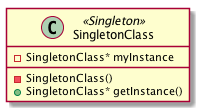
\includegraphics[height=3cm]{FSingleton.png}
\end{frame}
\begin{frame}[label={sec:orgheadline14}]{Strategy}
\begin{itemize}
\item Problem: \emph{There are different ways of doing the same thing; I want an extensible way of selecting between them.}
\item Solution: \emph{Use polymorphism to implement each different way.}
\item Example:
\end{itemize}

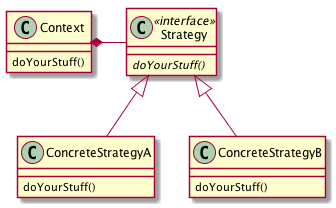
\includegraphics[height=4cm]{FStrategy.png}

(A more concrete example: Spellcheckers)
\end{frame}

\begin{frame}[label={sec:orgheadline15}]{State}
\begin{itemize}
\item Problem: \emph{You have a stateful system and want this to be mimicked by your class structure}
\item Solution: \emph{Implement it as a strategy pattern}
\item Example:
\end{itemize}
\end{frame}
\begin{frame}[label={sec:orgheadline16}]{Example: State Diagram}
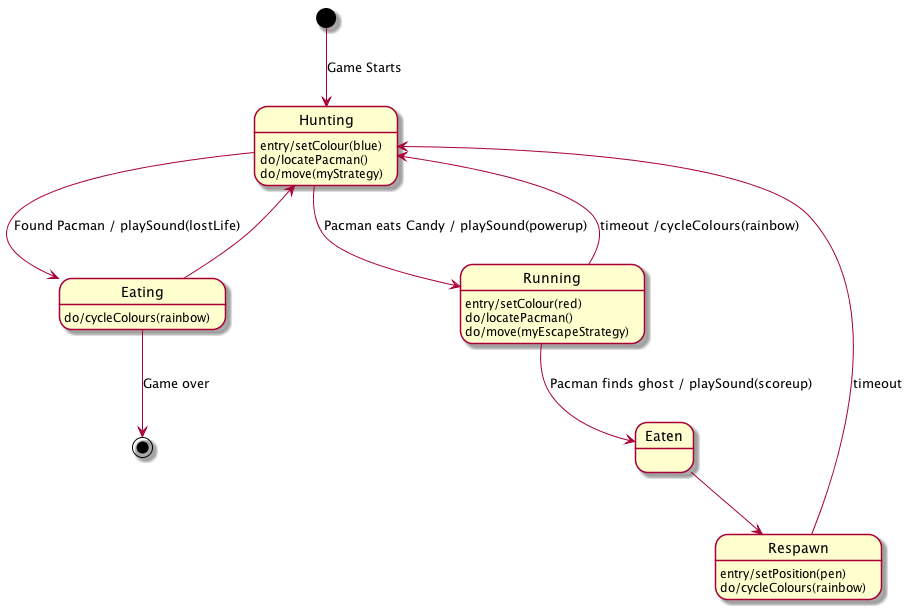
\includegraphics[height=6cm]{FState0.png}
\end{frame}
\begin{frame}[label={sec:orgheadline17}]{Example: Class Diagram}
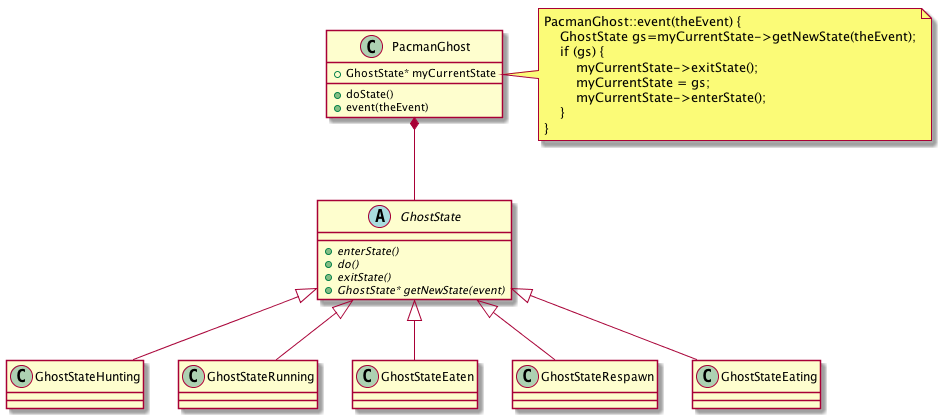
\includegraphics[height=6cm]{FState1.png}
\end{frame}

\begin{frame}[label={sec:orgheadline18}]{Abstract Factory}
\begin{itemize}
\item Problem: \emph{There are different ways to initiate the system, depending on the context}
\item Solution: \emph{Use a strategy-like solution to create the right objects}
\item Example:
\end{itemize}
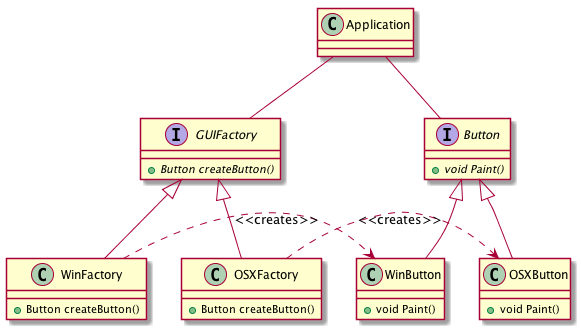
\includegraphics[height=4cm]{FAbstractFactory.png}
\end{frame}
\end{document}